\begin{itemize}
    \item La clasificación es fundamental tanto para la inteligencia humana como para la artificial.
    \item Decidir qué letra, palabra o imagen se ha presentado a nuestros sentidos, reconocer caras o voces, clasificar el correo, asignar calificaciones a las tareas.
    \item Estos son ejemplos de asignar una categoría a una entrada.
    \item El objetivo de la clasificación es tomar una única observación, extraer algunas características útiles y así clasificar la observación en una de las clases discretas establecidas.
    \item La mayoría de los casos de clasificación en el procesamiento del lenguaje se realizan mediante aprendizaje automático supervisado.
    \item Estas diapositivas se basan en el material del curso de Daniel Jurafsky: \url{https://web.stanford.edu/~jurafsky/slp3/4.pdf}
\end{itemize}

Ejemplo 1: Clasificación de spam

\begin{figure}[h]

\includegraphics[scale = 0.35]{pics/spam.png}
\end{figure}


Ejemplo 2: ¿Quién escribió los documentos Federalist?

\begin{itemize}
    \item 1787-8: Ensayos anónimos intentaron convencer a Nueva York de ratificar la Constitución de EE. UU.: Jay, Madison, Hamilton.
    \item La autoría de 12 de las cartas está en disputa.
    \item 1963: Resuelto por Mosteller y Wallace mediante métodos bayesianos.
\end{itemize}

\begin{center}
    \begin{figure}[h]
        \begin{minipage}{0.3\textwidth}
            \centering
            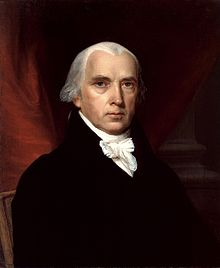
\includegraphics[width=\linewidth]{pics/madison.png}
            \caption{James Madison}
        \end{minipage}\hfill
        \begin{minipage}{0.3\textwidth}
            \centering
            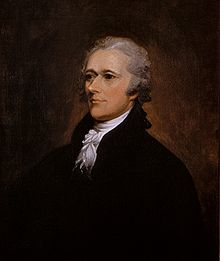
\includegraphics[width=\linewidth]{pics/hamilton.png}
            \caption{Alexander Hamilton}
        \end{minipage}
    \end{figure}
\end{center}


Ejemplo 3: ¿Cuál es el tema de este artículo médico?

\begin{figure}[h]
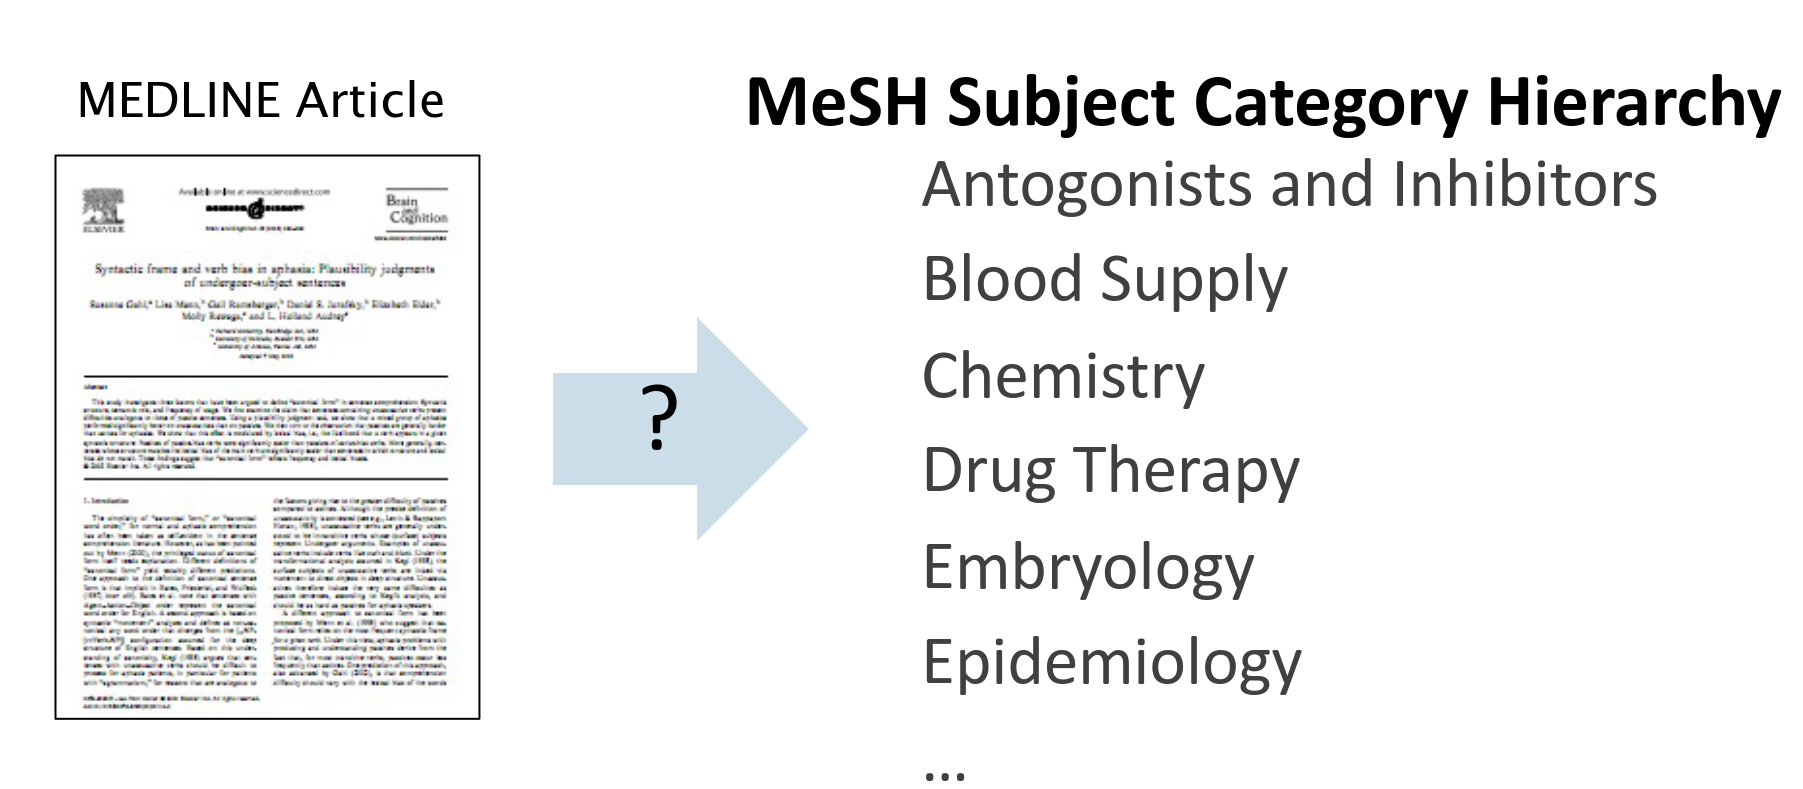
\includegraphics[scale = 0.2]{pics/medarticle.png}
\end{figure}



Ejemplo 4: ¿Reseña de película positiva o negativa?

\begin{itemize}
    \item \textcolor{blue}{\textbf{+}} ...personajes extravagantes y sátira \textcolor{blue}{rico} aplicada, y algunos \textcolor{blue}{grandes} giros de la trama.
    \item \textcolor{red}{\textbf{-}} Fue \textcolor{red}{patético}. La peor parte fue las escenas de boxeo...
    \item \textcolor{blue}{\textbf{+}} ...salsa de caramelo \textcolor{blue}{increíble} y almendras dulces y tostadas. ¡Me \textcolor{blue}{encanta} este lugar!
    \item \textcolor{red}{\textbf{-}} ...pizza \textcolor{red}{horrible} y \textcolor{red}{ridículamente} cara...
\end{itemize}



\paragraph{¿Por qué el análisis de sentimientos?}

\begin{itemize}
    \item Película: ¿Esta reseña es positiva o negativa?
    \item Productos: ¿Qué opinan las personas sobre el nuevo iPhone?
    \item Sentimiento público: ¿Cómo está la confianza del consumidor?
    \item Política: ¿Qué opinan las personas sobre este candidato o tema?
    \item Predicción: Predecir resultados electorales o tendencias del mercado a partir del sentimiento.
\end{itemize}


\paragraph{Clasificación básica de sentimientos}

El análisis de sentimientos es la detección de actitudes.

\begin{itemize}
    \item Tarea simple en la que nos enfocamos en esta clase.
    \begin{itemize}
        \item ¿Es la actitud de este texto positiva o negativa?
    \end{itemize}
\end{itemize}



\paragraph{Resumen: Clasificación de texto}

La clasificación de texto se puede aplicar a varias tareas, incluyendo:

\begin{itemize}
    \item Análisis de sentimientos
    \item Detección de spam
    \item Identificación de autoría
    \item Identificación de idioma
    \item Asignación de categorías, temas o géneros
    \item ...
\end{itemize}


\section{Clasificación de texto: Definición}

\textbf{Entrada}:
\begin{itemize}
    \item Un documento $d$
    \item Un conjunto fijo de clases $C = \{c_1, c_2, \ldots, c_J\}$
\end{itemize}

\textbf{Salida}: Una clase predicha $c \in C$


\subsection{Métodos de clasificación: Reglas codificadas a mano}

Reglas basadas en combinaciones de palabras u otras características.

\begin{itemize}
    \item Spam: \textit{dirección-en-lista-negra} O (\textit{“dólares” Y “has sido seleccionado”})
    \item La precisión puede ser alta si las reglas se refinan cuidadosamente por expertos
    \item Pero construir y mantener estas reglas es costoso
\end{itemize}

\subsection{Métodos de clasificación: Aprendizaje automático supervisado}

\textbf{Entrada}:
\begin{itemize}
    \item Un documento $d$
    \item Un conjunto fijo de clases $C = \{c_1, c_2, \ldots, c_J\}$
    \item Un conjunto de entrenamiento de $m$ documentos etiquetados manualmente: $(d_1, c_1), (d_2, c_2), \ldots, (d_m, c_m)$
\end{itemize}

\textbf{Salida}:
\begin{itemize}
    \item Un clasificador aprendido $\gamma: d \to c$
\end{itemize}

Cualquier tipo de clasificador se puede utilizar:
\begin{itemize}
    \item Naïve Bayes
    \item Regresión logística
    \item Redes neuronales
    \item k-vecinos más cercanos
    % Agrega más clasificadores según sea necesario
\end{itemize}

\subsection{Problemas de aprendizaje supervisado}
\begin{itemize}
    \item Tenemos ejemplos de entrenamiento $x^{(i)}$, $y^{(i)}$ para $i = 1, \ldots, m$. Cada $x^{(i)}$ es una entrada, cada $y^{(i)}$ es una etiqueta.
    \item La tarea es aprender una función $f$ que asigna las entradas $x$ a las etiquetas $f(x)$.
    \item Modelos condicionales:
    \begin{itemize}
        \item Aprender una distribución $p(y|x)$ a partir de ejemplos de entrenamiento.
        \item Para cualquier entrada de prueba $x$, definir $f(x) = \arg \max_y p(y|x)$.
    \end{itemize}
\end{itemize}

\subsection{Modelos generativos}
\begin{itemize}
    \item Dados ejemplos de entrenamiento $x^{(i)}$, $y^{(i)}$ para $i = 1, \ldots, m$, la tarea es aprender una función $f$ que asigna las entradas $x$ a las etiquetas $f(x)$.
    \item Modelos generativos:
    \begin{itemize}
        \item Aprender la distribución conjunta $p(x, y)$ a partir de los ejemplos de entrenamiento.
        \item A menudo, tenemos $p(x, y) = p(y)p(x|y)$.
        \item Nota: Luego tenemos
        \[
        p(y|x) = \frac{p(y)p(x|y)}{p(x)} \quad \text{donde} \quad p(x) = \sum_y p(y)p(x|y).
        \]
    \end{itemize}
\end{itemize}

\subsection{Clasificación con Modelos Generativos}
\begin{itemize}
    \item Dados ejemplos de entrenamiento $x^{(i)}$, $y^{(i)}$ para $i = 1, \ldots, m$. La tarea consiste en aprender una función $f$ que mapee las entradas $x$ a las etiquetas $f(x)$.
    \item Modelos generativos:
    \begin{itemize}
        \item Aprenden la distribución conjunta $p(x, y)$ a partir de los ejemplos de entrenamiento.
        \item A menudo, tenemos $p(x, y) = p(y)p(x|y)$.
    \end{itemize}
    \item La salida del modelo es:
    \[
    \begin{aligned}
    f(x) = \arg\max_y p(y|x) &= \arg\max_y \frac{p(y)p(x|y)}{p(x)} \\
    &= \arg\max_y p(y)p(x|y)
    \end{aligned}
    \]
\end{itemize}


\section{Intuición del Bayes Ingenuo}
El Bayes Ingenuo es un método de clasificación simple ("ingenuo") basado en la regla de Bayes.
\begin{itemize}
    \item Se basa en una representación muy simple de un documento: \textit{Bolsa de palabras}.
\end{itemize}



\subsection{Aplicación de la Regla de Bayes a Documentos y Clases}
Para un documento $d$ y una clase $c$:
\[
P(c | d) = \frac{P(d | c)P(c)}{P(d)}
\]


\section{Clasificador Bayes Ingenuo}
\begin{itemize}
    \item MAP significa ``máximo a posteriori'', que representa la clase más probable:
    \[
    c_{\text{MAP}} = \arg\max_{c \in C} P(c | d)
    \]
    \item Para calcular la clase más probable, aplicamos la regla de Bayes:
    \[
    = \arg\max_{c \in C} \frac{P(d | c)P(c)}{P(d)}
    \]
    \item Finalmente, podemos eliminar el denominador ya que permanece constante para todas las clases:
    \[
    = \arg\max_{c \in C} P(d | c)P(c)
    \]
    \item Para clasificar el documento $d$, usamos la estimación MAP:
    \[
    c_{\text{MAP}} = \arg\max_{c \in C} P(d | c)P(c)
    \]
    \item El documento $d$ se representa como un conjunto de características $x_1, x_2, \ldots, x_n$.
    \item El clasificador calcula la probabilidad condicional de las características dada una clase y la probabilidad a priori de la clase:
    \[
    = \arg\max_{c \in C} P(x_1, x_2, \ldots, x_n | c)P(c)
    \]
    \item El término $P(x_1, x_2, \ldots, x_n | c)$ representa la

 "verosimilitud" de las características dada la clase.
    \item El término $P(c)$ representa la probabilidad "a priori" de la clase.
    \item El clasificador Bayes Ingenuo \cite{mccallum1998comparison} calcula la estimación MAP considerando las probabilidades de verosimilitud y a priori:
    \[
    c_{\text{MAP}} = \arg\max_{c \in C} P(x_1, x_2, \ldots, x_n | c)P(c)
    \]
    \item La probabilidad de las características dada la clase, $P(x_1, x_2, \ldots, x_n | c)$, puede estimarse contando las frecuencias relativas en un corpus.
    \item La probabilidad a priori de la clase, $P(c)$, representa con qué frecuencia ocurre esta clase.
    \item Sin algunas suposiciones simplificadoras, estimar la probabilidad de cada posible combinación de características en $P(x_1, x_2, \ldots, x_n | c)$ requeriría un gran número de parámetros y conjuntos de entrenamiento imposiblemente grandes.
    \item Por lo tanto, los clasificadores Bayes Ingenuo realizan dos suposiciones simplificadoras.
\end{itemize}


\subsection{Suposiciones de Independencia del Bayes Ingenuo Multinomial}
\begin{itemize}
    \item Suposición de Bolsa de Palabras: asumimos que la posición de las palabras en el documento no importa.
    \item Suposición de Independencia Condicional: asumimos que las probabilidades de las características $P(x_i | c_j)$ son independientes dada la clase $c_j$.
    \item En el clasificador Bayes Ingenuo Multinomial, la probabilidad de un documento con características $x_1, x_2, \ldots, x_n$ dada la clase $c$ se puede calcular como:
    \[
    P(x_1, x_2, \ldots, x_n | c) = P(x_1 | c) \cdot P(x_2 | c) \cdot P(x_3 | c) \cdot \ldots \cdot P(x_n | c)
    \]
\end{itemize}

\subsection{Clasificador Bayes Ingenuo Multinomial}
\begin{itemize}
    \item La estimación del Máximo A Posteriori (MAP) para la clase $c$ en el clasificador Bayes Ingenuo Multinomial se calcula como:
    \[
    c_{\text{MAP}} = \arg\max_{c \in C} P(x_1, x_2, \ldots, x_n | c)P(c)
    \]
    \item Alternativamente, podemos escribirlo como:
    \[
    c_{\text{NB}} = \arg\max_{c \in C} P(c_j) \prod_{x \in X} P(x | c)
    \]
    \item $P(c_j)$ representa la probabilidad a priori de la clase $c_j$.
    \item $\prod_{x \in X} P(x | c)$ representa la verosimilitud de las características $x_1, x_2, \ldots, x_n$ dadas la clase $c$.
\end{itemize}


\subsection{Aplicación de los clasificadores Naive Bayes multinomiales a la clasificación de texto}

El clasificador Naive Bayes multinomial para la clasificación de texto se puede aplicar de la siguiente manera:
\[
c_{\text{NB}} = \arg\max_{c_j \in C} P(c_j) \prod_{i \in \text{positions}} P(x_i | c_j)
\]
Donde:
\begin{itemize}
    \item $c_{\text{NB}}$ representa la clase predicha para el documento de prueba.
    \item $C$ es el conjunto de todas las clases posibles.
    \item $P(c_j)$ es la probabilidad previa de la clase $c_j$.
    \item $\prod_{i \in \text{positions}} P(x_i | c_j)$ calcula la probabilidad de cada característica $x_i$ en la posición $i$ dada la clase $c_j$.
    \item El producto se toma sobre todas las posiciones de palabras en el documento de prueba.
\end{itemize}

\subsection{Problemas al multiplicar muchas probabilidades}

Multiplicar muchas probabilidades puede resultar en un desbordamiento de punto flotante, especialmente cuando se manejan probabilidades pequeñas. Por ejemplo, $0.0006 \times 0.0007 \times 0.0009 \times 0.01 \times 0.5 \times 0.000008 \ldots$.

Para solucionar este problema, podemos utilizar logaritmos, ya que $\log(ab) = \log(a) + \log(b)$. En lugar de multiplicar las probabilidades, podemos sumar los logaritmos de las probabilidades. Así, el clasificador Naive Bayes multinomial se puede expresar utilizando logaritmos de la siguiente manera:
\[
c_{\text{NB}} = \arg\max_{c_j \in C} \left(\log(P(c_j)) + \sum_{i \in \text{position}} \log(P(x_i | c_j))\right)
\]

Al tomar logaritmos, evitamos el problema del desbordamiento de punto flotante y realizamos cálculos en el espacio logarítmico. El clasificador se convierte en un modelo lineal, donde la predicción es el argmax de la suma de pesos (logaritmos de probabilidades) y las entradas (logaritmos de probabilidades condicionales). Por lo tanto, Naive Bayes es un clasificador lineal que opera en el espacio logarítmico.

\subsection{Aprendizaje del modelo Naive Bayes multinomial}

El primer intento: Estimaciones de máxima verosimilitud
\begin{itemize}
    \item Las probabilidades se estiman utilizando las frecuencias observadas en los datos de entrenamiento.
    \item La probabilidad previa de una clase $c_j$ se estima como:
    \[
    \hat{P}(c_j) = \frac{N_{c_j}}{N_{\text{total}}}
    \]
    donde $N_{c_j}$ es el número de documentos en la clase $c_j$ y $N_{\text{total}}$ es el número total de documentos.
    \item La estimación de la probabilidad de la palabra $w_i$ dada la clase $c_j$ se calcula como:
    \[
    \hat{P}(w_i | c_j) = \frac{{\text{count}(w_i, c_j)}}{\sum_{w\in V}{\text{count}(w, c_j)}}
    \]
    donde $w \in V$ representa una palabra en el vocabulario $V$.
    \item El denominador es la suma de las frecuencias de todas las palabras en el vocabulario dentro de la clase $c_j$.
\end{itemize}

\subsection{Estimación de parámetros}

Para estimar los parámetros del modelo Naive Bayes multinomial, seguimos estos pasos:

\begin{itemize}
  \item Creamos un mega-documento para cada tema $c_j$ concatenando todos los documentos de ese tema.
  \item Calculamos la frecuencia de la palabra $w_i$ en el mega-documento, que representa la fracción de veces que la palabra $w_i$ aparece entre todas las palabras en los documentos del tema $c_j$.
  \item La probabilidad estimada $\hat{P}(w_i | c_j)$ de la palabra $w_i$ dada la clase $c_j$ se obtiene dividiendo el recuento de ocurrencias de $w_i$ en el mega-documento del tema $c_j$ por el recuento total de palabras en el mega-documento:
  \[
  \hat{P}(w_i | c_j) = \frac{{\text{count}(w_i, c_j)}}{\sum_{w\in V}{\text{count}(w, c_j)}}
  \]
  Aquí, $\text{count}(w_i, c_j)$ representa el número de veces que la palabra $w_i$ aparece en el mega-documento del tema $c_j$, y $\text{count}(w, c_j)$ es el recuento total de palabras en el mega-documento.
\end{itemize}

\subsection{Probabilidades cero y el problema de las palabras no vistas}

Consideremos el escenario en el que no hemos encontrado la palabra "fantástico" en ningún documento de entrenamiento clasificado como positivo (pulgar hacia arriba). Utilizando la estimación de máxima verosimilitud, la probabilidad $\hat{P}(\text{``fantástico''} \mid \text{positivo})$ se calcularía como:
\[
\hat{P}(\text{``fantástico''} \mid \text{positivo}) = \frac{\text{count}(\text{``fantástico''}, \text{positivo})}{\sum_{w \in V} \text{count}(w, \text{positivo})}
\]

En este caso, el recuento de la palabra ``fantástico'' en los documentos positivos es cero, lo que conduce a una probabilidad cero:
\[
\hat{P}(\text{``fantástico''} \mid \text{positivo}) = \frac{0}{\sum_{w \in V} \text{count}(w, \text{positivo})} = 0
\]

Sin embargo, las probabilidades cero no pueden eliminarse, independientemente de la evidencia adicional presente. Esto plantea un problema al calcular la estimación del máximo a posteriori (MAP), que se utiliza para la clasificación:
\[
c_{\text{MAP}} = \arg\max_c \left(\hat{P}(c) \prod_{i} \hat{P}(x_i \mid c)\right)
\]

Con una probabilidad cero para una palabra, toda la expresión se vuelve cero, independientemente de la otra evidencia.

\subsection{Suavizado Laplaciano (Add-1) para Naïve Bayes}

Manejo de probabilidades cero con el suavizado Laplaciano (Add-1):
\begin{itemize}
    \item Para abordar el problema de las probabilidades cero, podemos utilizar la técnica de suavizado Laplaciano (Add-1).
    \item La estimación suavizada $\hat{P}(w_i \mid c)$ se calcula como:
    \[
    \hat{P}(w_i \mid c) = \frac{\text{count}(w_i, c) + 1}{\sum_{w \in V} (\text{count}(w, c) + 1)}
    \]
    \item Aquí, se agrega un recuento adicional de 1 tanto al numerador como al denominador.
    \item El denominador se ajusta agregando el tamaño del vocabulario $V$ para garantizar una normalización adecuada.
    \item Al hacerlo, evitamos las probabilidades cero y permitimos que cierta masa de probabilidad se distribuya a palabras no vistas.
    \item Esta técnica de suavizado ayuda a mitigar el problema de las palabras no vistas y evita la eliminación completa de ciertas clases durante la clasificación.
\end{itemize}

\subsection{Naïve Bayes multinomial: aprendizaje}

Aprendiendo el modelo Naïve Bayes multinomial:
\begin{itemize}
    \item Para aprender los parámetros del modelo, necesitamos calcular los términos $P(c_j)$ y $P(w_k \mid c_j)$.
    \item Para cada clase $c_j$ en el conjunto de clases $C$, realizamos los siguientes pasos:
    \begin{itemize}
        \item Recuperamos todos los documentos $docs_j$ que pertenecen a la clase $c_j$.
        \item Calculamos el término $P(w_k \mid c_j)$ para cada palabra $w_k$ en el vocabulario $V$:
        \[
        P(w_k \mid c_j) = \frac{{n_k + \alpha}}{{n + \alpha \cdot \lvert \text{Vocabulary} \rvert}}
        \]
        donde $n_k$ representa el número de ocurrencias de la palabra $w_k$ en el documento concatenado $Text_j$.
        \item Calculamos la probabilidad a priori $P(c_j)$:
        \[
        P(c_j) = \frac{{\lvert docs_j \rvert}}{{\lvert \text{total number of documents} \rvert}}
        \]
    \end{itemize}
    \item Para calcular $P(w_k \mid c_j)$, necesitamos extraer el vocabulario $V$ del corpus de entrenamiento.
\end{itemize}

\subsection{Palabras desconocidas}

Tratamiento de palabras desconocidas en los datos de prueba:
\begin{itemize}
    \item Cuando encontramos palabras desconocidas en los datos de prueba que no aparecen en los datos de entrenamiento o en el vocabulario, las ignoramos.
    \item Eliminamos estas palabras desconocidas del documento de prueba como si no estuvieran presentes en absoluto.
    \item No asignamos ninguna probabilidad a estas palabras desconocidas en el proceso de clasificación.
\end{itemize}

Esto es una visión general del modelo Naive Bayes multinomial y su aplicación a la clasificación de texto. Cabe destacar que existen variantes y extensiones más sofisticadas de Naive Bayes que se adaptan a diferentes requisitos y características de los datos.


\section{Ejemplo}

\textbf{Datos de Entrenamiento:} 

\begin{table}[h]
\centering
\begin{tabular}{|c|p{0.7\textwidth}|}
\hline
\textbf{Categoría} & \textbf{Texto} \\
\hline
Negative & Just plain boring, entirely predictable and lacks energy. \\
\hline
Negative & No surprises and very few laughs. \\
\hline
Positive & Very powerful. \\
\hline
Positive & The most fun film of the summer. \\
\hline
\end{tabular}
\end{table}


\textbf{Test:} 
\begin{table}[h]
\centering
\begin{tabular}{|c|p{0.7\textwidth}|}
\hline
\textbf{Categoría} & \textbf{Texto} \\
\hline
? & Predictable with no fun. \\
\hline
\end{tabular}
\end{table}

\begin{figure}[h]
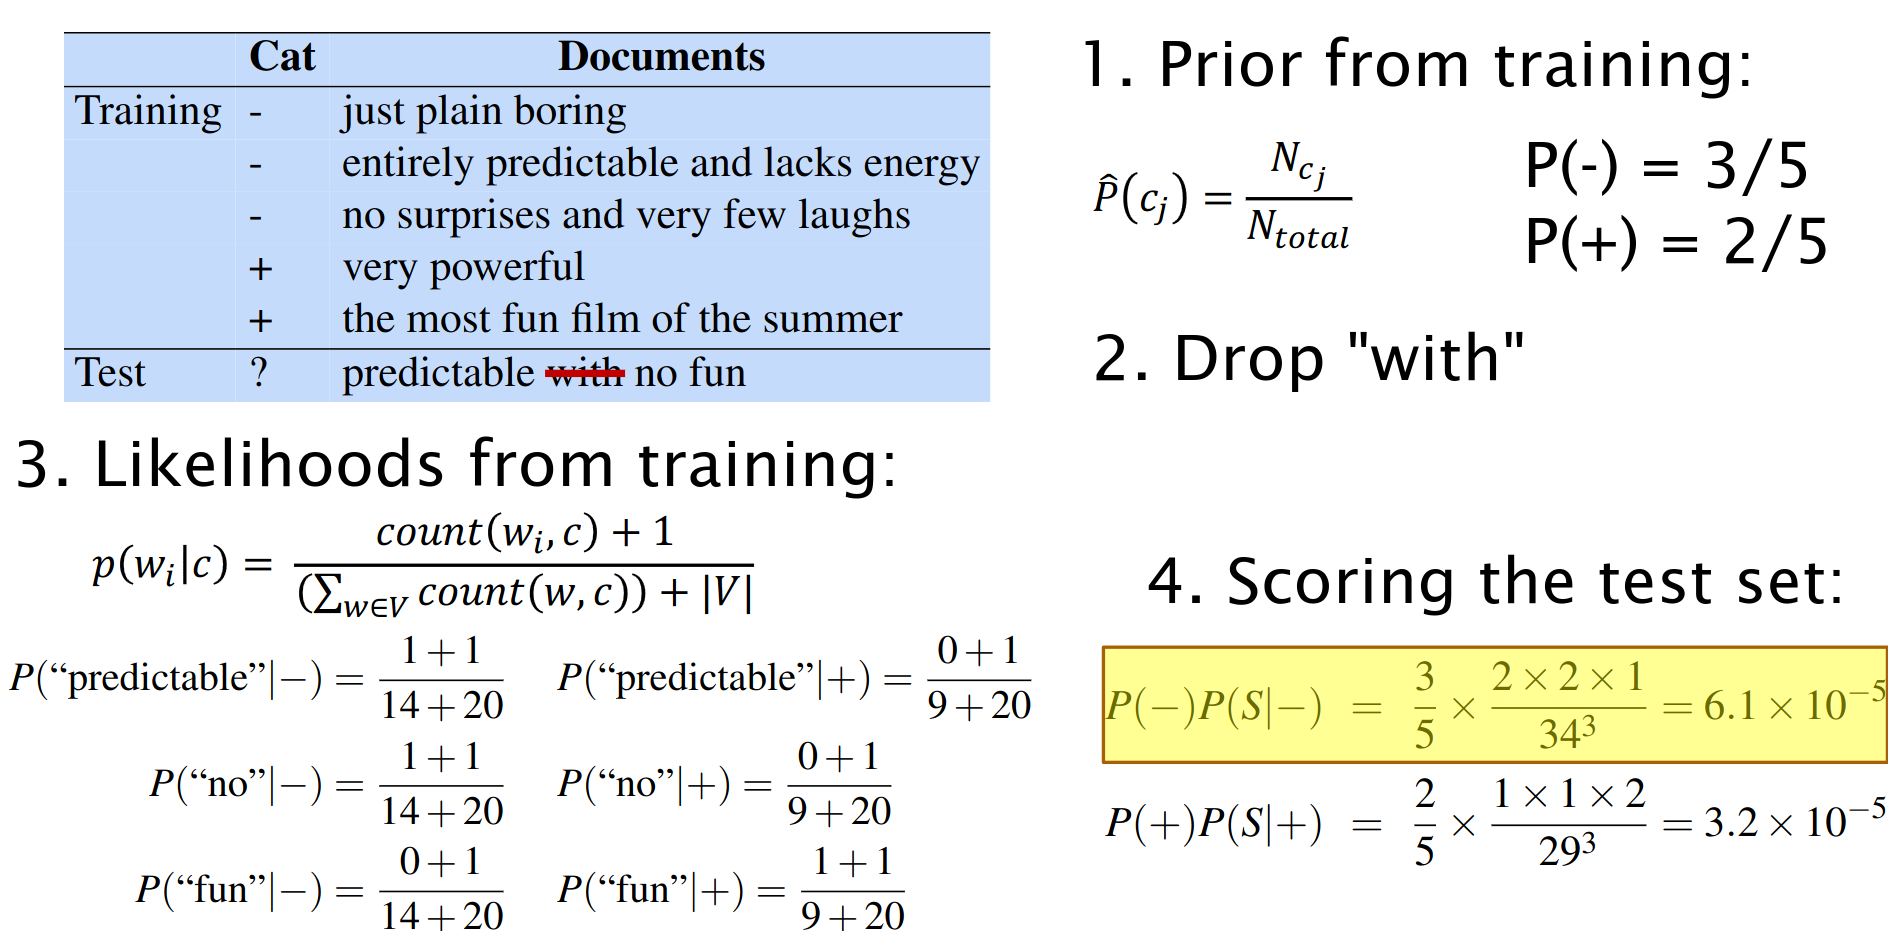
\includegraphics[scale = 0.23]{pics/naive_example.png}
\end{figure}

\section{Naive Bayes como modelo de lenguaje}

Cuando utilizamos características de palabras individuales y consideramos todas las palabras en el texto, el naive Bayes tiene una similitud importante con la modelización del lenguaje.

Específicamente, un modelo naive Bayes se puede ver como un conjunto de modelos de lenguaje de unigramas específicos de cada clase, en el que el modelo para cada clase instancia un modelo de lenguaje de unigrama.

Las características de verosimilitud del modelo naive Bayes asignan una probabilidad a cada palabra $P(\text{word}|c)$, y el modelo también asigna una probabilidad a cada oración:

\[P(s|c) = \prod_{i\in \text{positions}} P(w_i|c)\]

Consideremos un modelo naive Bayes con las clases positiva (+) y negativa (-) y los siguientes parámetros del modelo:

\begin{center}
\begin{tabular}{ccc}
\textbf{w} & $P(w|+)$ & $P(w|-)$ \\
I & 0.1 & 0.2 \\
love & 0.1 & 0.001 \\
this & 0.01 & 0.01 \\
fun & 0.05 & 0.005 \\
film & 0.1 & 0.1 \\
... & ... & ...
\end{tabular}
\end{center}

Cada una de las dos columnas anteriores instancian un modelo de lenguaje que puede asignar una probabilidad a la oración "I love this fun film":

\[P("\text{I love this fun film}"|+) = 0.1 \times 0.1 \times 0.01 \times 0.05 \times 0.1 = 0.0000005\]
\[P("\text{I love this fun film}"|-) = 0.2 \times 0.001 \times 0.01 \times 0.005 \times 0.1 = 0.0000000010\]

Como sucede, el modelo positivo asigna una probabilidad más alta a la oración:
\[P(s|\text{pos}) > P(s|\text{neg})\]

Cabe destacar que esto es solo la parte de verosimilitud del modelo naive Bayes; una vez que multiplicamos por la probabilidad a priori, un modelo naive Bayes completo podría tomar una decisión de clasificación diferente.



\section{Evaluación}

\begin{itemize}
 \item Consideremos solo tareas de clasificación de texto binario.
 \item Imagina que eres el CEO de Delicious Pie Company.
 \item Quieres saber lo que la gente está diciendo sobre tus pasteles.
 \item Por lo tanto, construyes un detector de tweets de "Delicious Pie" con las siguientes clases:
\begin{itemize}
\item Clase positiva: tweets sobre Delicious Pie Co.
\item Clase negativa: todos los demás tweets.
\end{itemize}
\end{itemize}



\subsection{La Matriz de Confusión 2x2}
\begin{table}[h]
\centering
\begin{tabular}{|c|c|c|}
\hline
\textbf{} & \textbf{Sistema Positivo} & \textbf{Sistema Negativo} \\
\hline
\textbf{Oro Positivo} & Verdadero Positivo (VP) & Falso Negativo (FN) \\
\hline
\textbf{Oro Negativo} & Falso Positivo (FP) & Verdadero Negativo (VN) \\
\hline
\end{tabular}
\end{table}

\textbf{Recall} (también conocido como \textbf{Sensibilidad} o \textbf{Tasa de Verdaderos Positivos}):
\[ \text{Recall} = \frac{VP}{VP + FN} \]

\textbf{Precisión}:
\[ \text{Precisión} = \frac{VP}{VP + FP} \]

\textbf{Exactitud}:
\[ \text{Exactitud} = \frac{VP + VN}{VP + FP + VN + FN} \]


\subsection{Evaluación: Exactitud}
¿Por qué no usamos la exactitud como nuestra métrica?

Imagina que vimos 1 millón de tweets:
\begin{itemize}
\item 100 de ellos hablaban sobre Delicious Pie Co.
\item 999,900 hablaban de otra cosa.
\end{itemize}

Podríamos construir un clasificador tonto que simplemente etiquete todos los tweets como "no sobre pasteles":
\begin{itemize}
\item ¡¡¡Obtendría una exactitud del 99.99\%!!! ¡¡¡Wow!!!
\item ¡Pero sería inútil! ¡No devuelve los comentarios que estamos buscando!
\end{itemize}

Por eso usamos precisión y recall en su lugar.

\subsection{Evaluación: Precisión y Recall}
\textbf{Precisión} mide el porcentaje de elementos que el sistema detectó (es decir, los elementos que el sistema etiquetó como positivos) que son realmente positivos (según las etiquetas de oro humanas).

\[
\text{Precisión} = \frac{\text{Verdaderos Positivos}}{\text{Verdaderos Positivos + Falsos Positivos}}
\]

\textbf{Recall} mide el porcentaje de elementos que el sistema identificó correctamente de todos los elementos que deberían haber sido identificados.

\[
\text{Recall} = \frac{\text{Verdaderos Positivos}}{\text{Verdaderos Positivos + Falsos Negativos}}
\]

\subsection{¿Por qué Precisión y Recall?}
Considera nuestro clasificador tonto de pasteles que simplemente etiqu

eta nada como "sobre pasteles".

\begin{itemize}
  \item Exactitud = 99.99\% (etiqueta correctamente la mayoría de los tweets como no relacionados con pasteles)
  \item Recall = 0 (no detecta ninguno de los 100 tweets relacionados con pasteles)
\end{itemize}

La precisión y el recall, a diferencia de la exactitud, enfatizan los verdaderos positivos:
\begin{itemize}
  \item Se centran en encontrar las cosas que se supone que debemos buscar.
\end{itemize}

\subsection{Una Medida Combinada: Medida F}
La medida F es un número único que combina la precisión (P) y el recall (R), definida como:
\[
F_\beta = \frac{(\beta^2+1)PR}{\beta^2P + R}
\]

La medida F, definida con el parámetro $\beta$, pondera diferencialmente la importancia del recall y la precisión.
\begin{itemize}
  \item $\beta > 1$ favorece al recall
  \item $\beta < 1$ favorece a la precisión
\end{itemize}

Cuando $\beta = 1$, la precisión y el recall son iguales, y tenemos la medida $F_1$ equilibrada:
\[
F_1 = \frac{2PR}{P + R}
\]

\subsection{Conjuntos de Prueba de Desarrollo ("Devsets")}

\begin{itemize}
 \item Para evitar el sobreajuste y proporcionar una estimación más conservadora del rendimiento, comúnmente utilizamos un enfoque de tres conjuntos: conjunto de entrenamiento, conjunto de desarrollo y conjunto de prueba.
\begin{figure}[h]
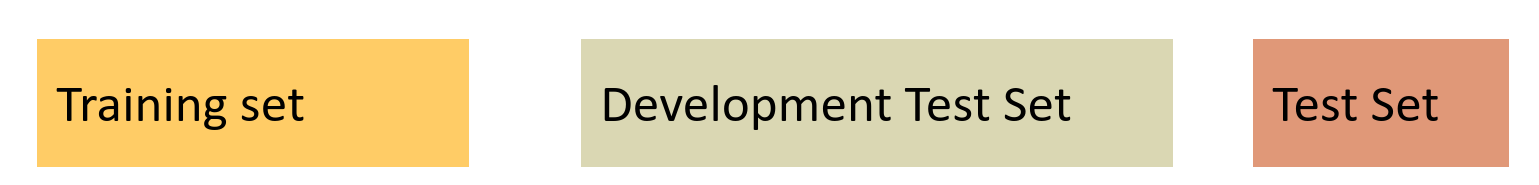
\includegraphics[scale = 0.23]{pics/devsets.png}
\end{figure}

\begin{itemize}
\item \textbf{Conjunto de entrenamiento}: Se utiliza para entrenar el modelo.
\item \textbf{Conjunto de desarrollo}: Se utiliza para ajustar el modelo y seleccionar los mejores hiperparámetros.
\item \textbf{Conjunto de prueba}: Se utiliza para informar el rendimiento final del modelo.
\end{itemize}

\item Este enfoque garantiza que el modelo no esté ajustado específicamente al conjunto de prueba, evitando el sobreajuste.
\item Sin embargo, crea una paradoja: queremos la mayor cantidad de datos posible para el entrenamiento, pero también para el conjunto de desarrollo.
\item ¿Cómo dividimos los datos?

\end{itemize}





\subsection{Validación Cruzada: Múltiples Divisiones}

\begin{itemize}
\item La validación cruzada nos permite utilizar todos nuestros datos para el entrenamiento y la prueba sin tener un conjunto de entrenamiento, conjunto de desarrollo y conjunto de prueba fijos.
\item Elegimos un número $k$ y dividimos nuestros datos en $k$ subconjuntos disjuntos llamados pliegues.
\item En cada iteración, uno de los pliegues se selecciona como conjunto de prueba mientras que los $k-1$ pliegues restantes se utilizan para entrenar el clasificador.
\item Calculamos la tasa de error en el conjunto de prueba y repetimos este proceso $k$ veces.
\item Finalmente, promediamos las tasas de error de estas $k$ ejecuciones para obtener una tasa de error promedio.
\item Por ejemplo, la validación cruzada de 10 pliegues implica entrenar 10 modelos con el 90\% de los datos y probar cada modelo por separado.
\item Las tasas de error resultantes se promedian para obtener la estimación final del rendimiento.
\item Sin embargo, la validación cruzada requiere que todo el corpus sea ciego, lo que impide examinar los datos para sugerir características o comprender el comportamiento del sistema.
\item Para abordar esto, se crea un conjunto de entrenamiento y un conjunto de prueba fijos, y se realiza la validación cruzada de 10 pliegues dentro del conjunto de entrenamiento.
\item La tasa de error se calcula convencionalmente en el conjunto de prueba.
\end{itemize}


\begin{center}
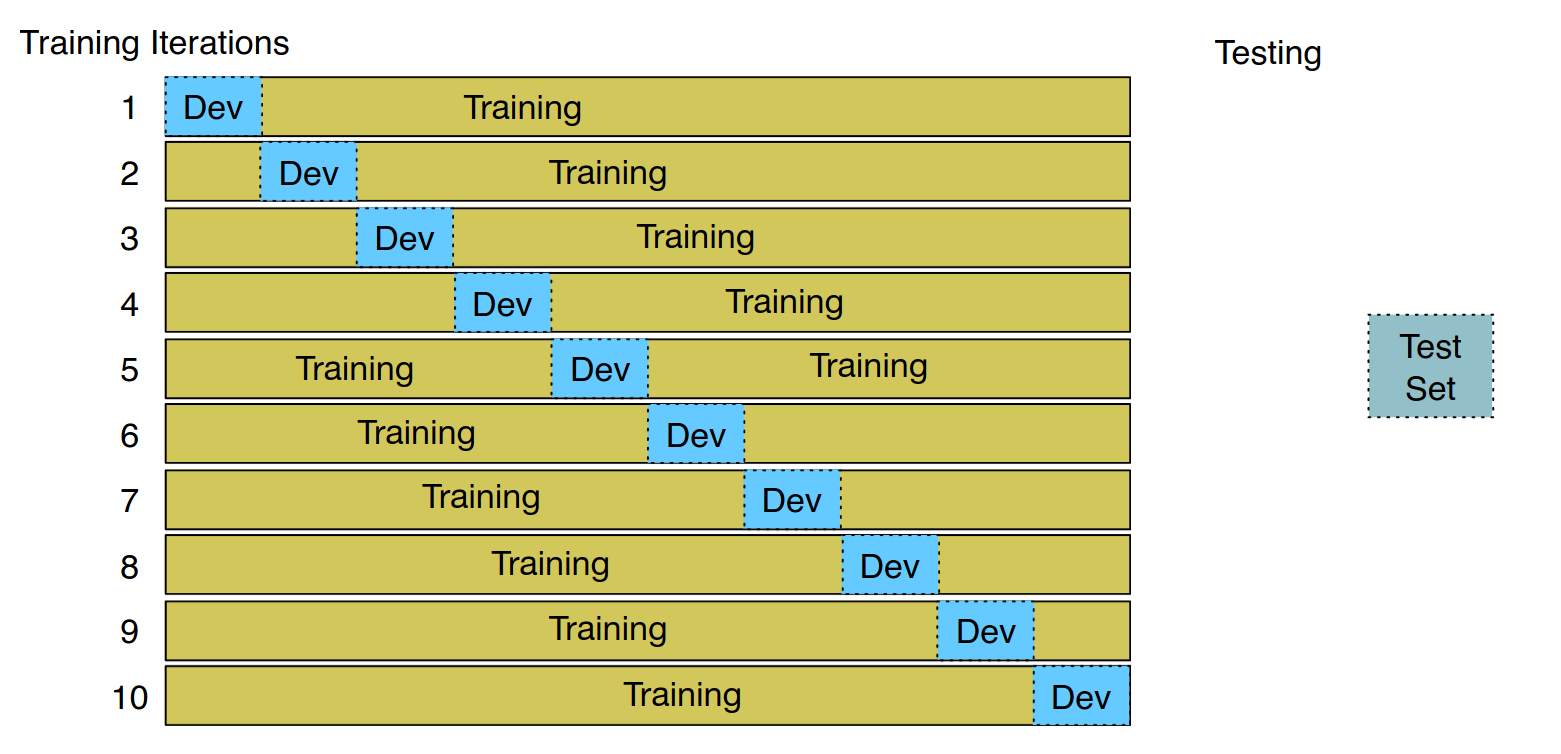
\includegraphics[scale=0.28]{pics/cv.png}
\end{center}


\subsection{Matriz de Confusión para clasificación de 3 clases}


\begin{center}
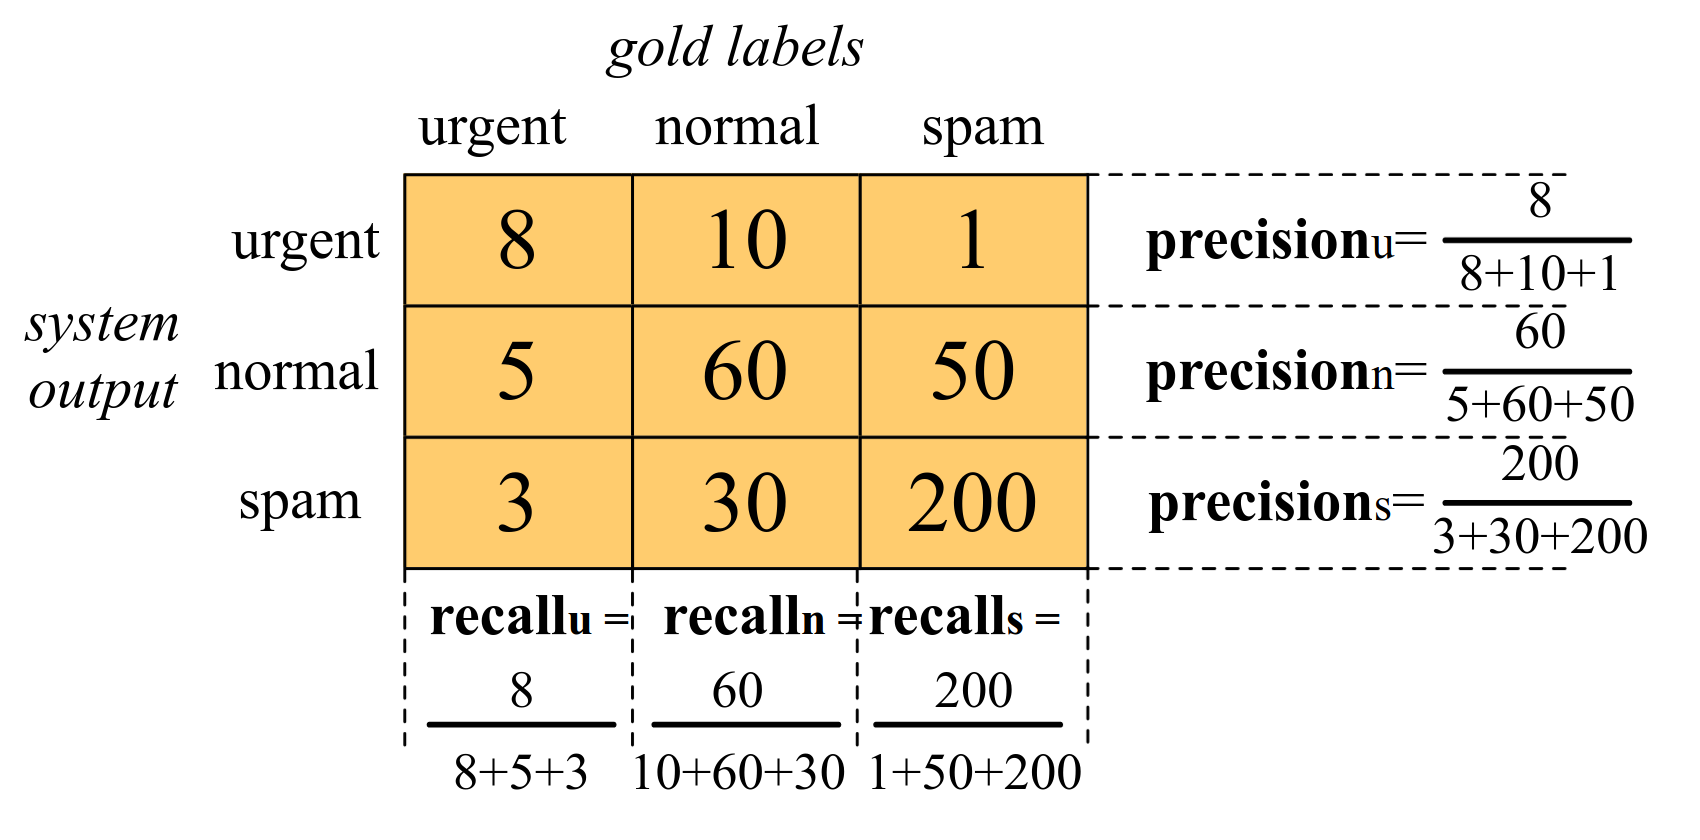
\includegraphics[scale=0.23]{pics/confmatrix.png}
\end{center}

Cómo combinar métricas binarias (Precisión, Recall, $F_1$) de más de 2 clases para obtener una métrica única:
\begin{itemize}
 \item Macro-promedio:
 \begin{itemize}
    \item Calcular las métricas de rendimiento (Precisión, Recall, $F_1$) para cada clase individualmente.
    \item Promediar las métricas en todas las clases.
 \end{itemize}
 \item Micro-promedio:
 \begin{itemize}
    \item Recopilar las decisiones para todas las clases en una matriz de confusión.
    \item Calcular la Precisión y el Recall a partir de la matriz de confusión.
 \end{itemize}
\end{itemize}

\begin{center}
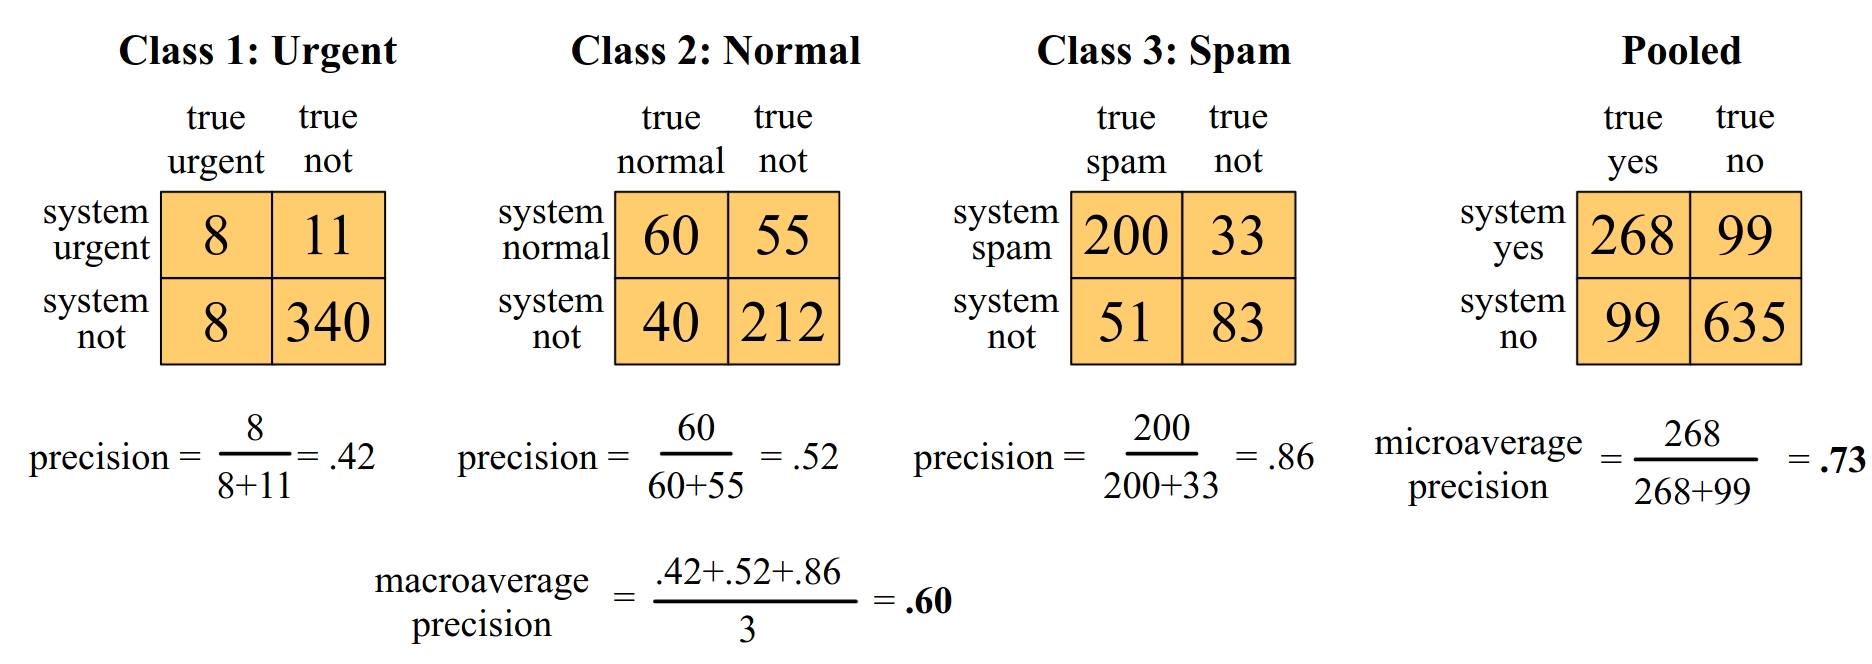
\includegraphics[scale=0.23]{pics/confmatrixmulti.png}
\end{center}
